\documentclass[12pt]{ctexart}
    %%% Document Settings %%%%
%\usepackage[utf8]{inputenc}

\usepackage[
    twoside,
    top=1in,
    bottom=0.75in,
    inner=0.5in,
    outer=0.5in,
]{geometry}
\pagestyle{myheadings}
\usepackage{minted}
\usepackage[dvipsnames,svgnames]{xcolor}

%%%% Additional Commands to Load %%%%
\usepackage{tcolorbox}
\tcbuselibrary{skins}
\tcbuselibrary{minted}
\usemintedstyle{lovelace}
%\usepackage{minted}
\usepackage{color}
\usepackage{tikz}
\usetikzlibrary{calc}
\usepackage{tabularx,colortbl}
\usepackage{amsfonts,amsmath,amssymb}
\usepackage{titling}
\usepackage{mathrsfs}
\usepackage{calc}
\usepackage{subcaption}

\usepackage{listings}
%\usepackage{newtxtext}
\usepackage[strict]{changepage} 
\usepackage{framed}
\definecolor{formalshade}{rgb}{0.95,0.95,1}
\usepackage{float}

%%%% Commands to Define Homework Boxes %%%%
%%%% Box Definition %%%%
\newtcolorbox{prob}[1]{
% Set box style
    sidebyside,
    sidebyside align=top,
% Dimensions and layout
    width=\textwidth,
    toptitle=2.5pt,
    bottomtitle=2.5pt,
    righthand width=0.20\textwidth,
% Coloring
    colbacktitle=gray!30,
    coltitle=black,
    colback=white,
    colframe=black,
% Title formatting
    title={
        #1 \hfill Grade:\phantom{WWWW}
    },
    fonttitle=\large\bfseries
}

%%%% Environment Definition %%%%
\newenvironment{problem}[1]{
    \begin{prob}{#1}
}
{
    \tcblower
    \centering
    \textit{\scriptsize\bfseries Faculty Comments}
    \vspace{\baselineskip}
    \end{prob}
}

\newenvironment{formal}{%
\def\FrameCommand{%
\hspace{1pt}%
{\color{DarkBlue}\vrule width 2pt}%
{\color{formalshade}\vrule width 4pt}%
\colorbox{formalshade}%
}%
\MakeFramed{\advance\hsize-\width\FrameRestore}%
\noindent\hspace{-4.55pt}% disable indenting first paragraph
\begin{adjustwidth}{}{7pt}%
\vspace{2pt}\vspace{2pt}%
}
{%
\vspace{2pt}\end{adjustwidth}\endMakeFramed%
}

    \title{特殊方程作业6}
    \author{地物2201班\ 杨曜堃}
    \date{\today}
%%% document
\begin{document}

% Format Running Header
    \markboth{\theauthor}{\thetitle}
    \maketitle
    \begin{description}
        \item[问题1] 考虑满足下列边界条件及初始条件的一维热传导方程:
        $$
        \begin{cases}
            \dfrac{\partial u}{\partial t}=\dfrac{\partial^2u}{\partial x^2},&\quad 0<x<1,\ t>0\\
            u|_{x=0}=100,\ u|_{x=1}=100,&\quad t\geqslant0\\
            u|_{t=0}=3\sin(5\pi x)+100,&\quad 0\leqslant x\leqslant 1

        \end{cases}
        $$
        \begin{enumerate}
            \item 采用分离变量法求解该定解问题;
            \item 验证上一步求得的$u(x,t)$满足定解问题。
        \end{enumerate}
    \end{description}

    % \begin{center}
    %     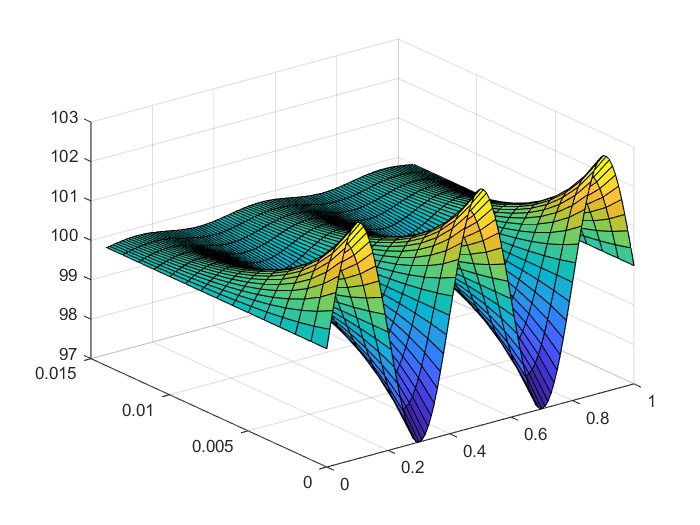
\includegraphics[width=16cm]{fig1.png}
    % \end{center}   
    \begin{problem}{问题\#1.1}
        考虑到非齐次边界条件的具体形式,可设齐次化函数为
        $$
        v(x)=100
        $$
        于是令
        $$
        u(x,t)=v(x)+w(x,t)=w(x,t)+100
        $$
        则有
        $$
        \dfrac{\partial w}{\partial t}=\dfrac{\partial^2w}{\partial x^2}
        $$
        对应的定解问题为
        $$
        \begin{cases}
            \dfrac{\partial w}{\partial t}=\dfrac{\partial^2w}{\partial x^2},&\quad 0<x<1,\ t>0\\
            w|_{x=0}=w|_{x=1}=0,&\quad t\geqslant 0\\
            w|_{t=0}=3\sin(5\pi x),&\quad 0\leqslant x\leqslant 1
        \end{cases}
        $$
    \end{problem}
    \begin{problem}{问题\#1.1}
        采用分离变量法,可得
        $$
        w(x,t)=\sum^{\infty}_{n=1}C_n\sin(n\pi x)e^{-(n\pi)^2t}
        $$
        代入初始条件
        $$
        w(x,0)=\sum^{\infty}_{n=1}C_n\sin(n\pi x)=3\sin(5\pi x)
        $$
        于是可以取$C_5=3$,
        $$
        w(x,t)=3\sin(5\pi x)e^{-(5\pi)^2t}
        $$
        问题的形式解为
        $$
        u(x,t)=3\sin(5\pi x)e^{-(5\pi)^2t}
        +100
        $$
    \end{problem}
    \newpage
    \begin{problem}{问题\#1.2}
        经验证,解得的$u(x,t)$是满足边界条件和初始条件的一解。
    \end{problem}
    MATLAB计算代码如下,用于图示辅助验证。
    \begin{lstlisting}[language = Matlab,title={test6\_script.m},  numbers=left, 
        numberstyle=\tiny,keywordstyle=\color{blue!70},
        commentstyle=\color{red!50!green!50!blue!50},frame=shadowbox,
        rulesepcolor=\color{red!20!green!20!blue!20},basicstyle=\ttfamily]
    % 图示求解结果
    clear;
            
    % 定义参数
    x = 0:0.1:1;
    t = 0:0.1:1;
    [X,T]=meshgrid(x,t);
        
    uxt = 3*sin(5*pi*X).*exp(-(5*pi)^2*T)+100;
        
    % 绘制图像
    figure;
    contourf(X,T,uxt,20);
    colorbar;
    xlabel('x');
    ylabel('t');
    \end{lstlisting}
    \begin{figure}[htbp]
        \small
        \centering
        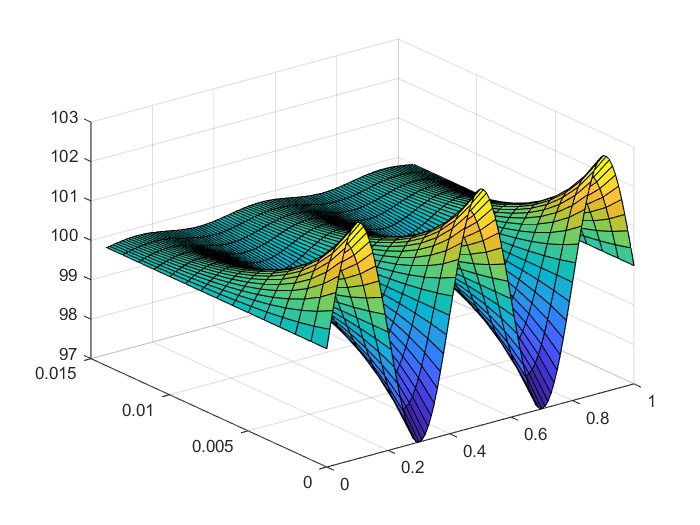
\includegraphics[width=16cm]{fig1.png}
        \caption{结果图示} \label{Fig:aa}
    \end{figure}
\end{document}